\documentclass[../../main.tex]{subfiles}

\begin{document}
\section{Calcolo vettoriale}
\subsection{Grandezze scalari e vettoriali}
Le grandezze scalari sono quelle che si possono rappresentare con un numero (temperatura, numero dei piedi), mentre quelle vettoriali sono grandezze che esprimono con tre numeri uno spostamento per esempio.
\subsubsection{Richiami di Analisi}
Differenziale:
\[
    df = f'(x)dx
\]
Svilippi di Taylor:
\[
    f(x) = f(x_0) + \dfrac{df}{dx} (x-x_0) + \ldots \ \ \ \textit{che solitamente in fisica si rimuovo perchè piccolossimi}
\]
Integrali doppi e equazioni differenziali.
\subsection{Vettori}
Quando si parla di vettori è importante indicare la \textbf{direzione} (la retta sulla quale ci si muove), il \textbf{verso} (la freccia) e il \textbf{modulo} (la lunghezza). Il vettore si chiama \textbf{applicato} se si indica la sua origine.
\subsubsection{Operazioni con i vettori}
\begin{itemize}
    \item \textbf{Prodotto di un vettore per uno scalare}: stessa direzione, stesso verso e modulo moltiplicato per lo scalare. $\vec{a} = \lambda \vec{b} : \lambda \in \mathbb{R}$
    \item \textbf{Versore}: vettore che ha la stessa direzione e verso di un vettore $\vec{a}$ ma modulo $1$. Si indica con $\bar{u}_a$
    \item \textbf{Vettore nullo}: vettore con modulo $0$, di cui non si può dire né direzione né verso. Si può ottenere sommando un vettore con il suo opposto. $\vec{a} + (-\vec{a}) = \vec{0}$
    \item \textbf{Vettore opposto}: vettore con la stessa direzione e verso ma modulo opposto. $\vec{a} + (-\vec{a}) = \vec{0}$
    \item \textbf{Regola del parallelogramma (somma)}: se si sommano due vettori si può ottenere il vettore risultante disegnando un parallelogramma con i due vettori come lati.
    \begin{figure}[h!]
        \centering
        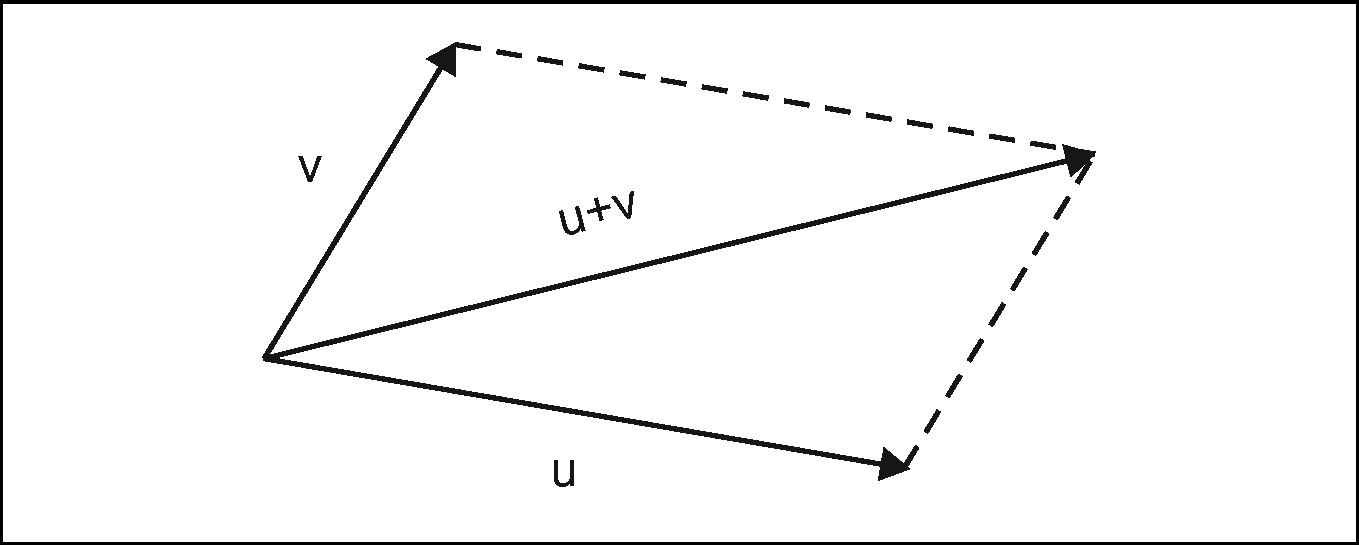
\includegraphics[width=0.5\textwidth]{parallelogramma.jpeg}
        \caption{Regola del parallelogramma}
    \end{figure}
\end{itemize}
\subsubsection{Proprietà dei vettori}
\begin{itemize}
    \item \textbf{Commutativa}: $\vec{a} + \vec{b} = \vec{b} + \vec{a}$
    \item \textbf{Differenza di vettori}: $\vec{a} - \vec{b} = \vec{a} + (-\vec{b})$. Per sottrarre un vettore devo cambiare il verso del vettore che sto sottraendo.
    \item \textbf{Somma di più vettori}: vale la proprietà \textbf{associativa}. $\vec{a} + (\vec{b} + \vec{c}) = (\vec{a} + \vec{b}) + \vec{c}$ \begin{figure}
        \centering
        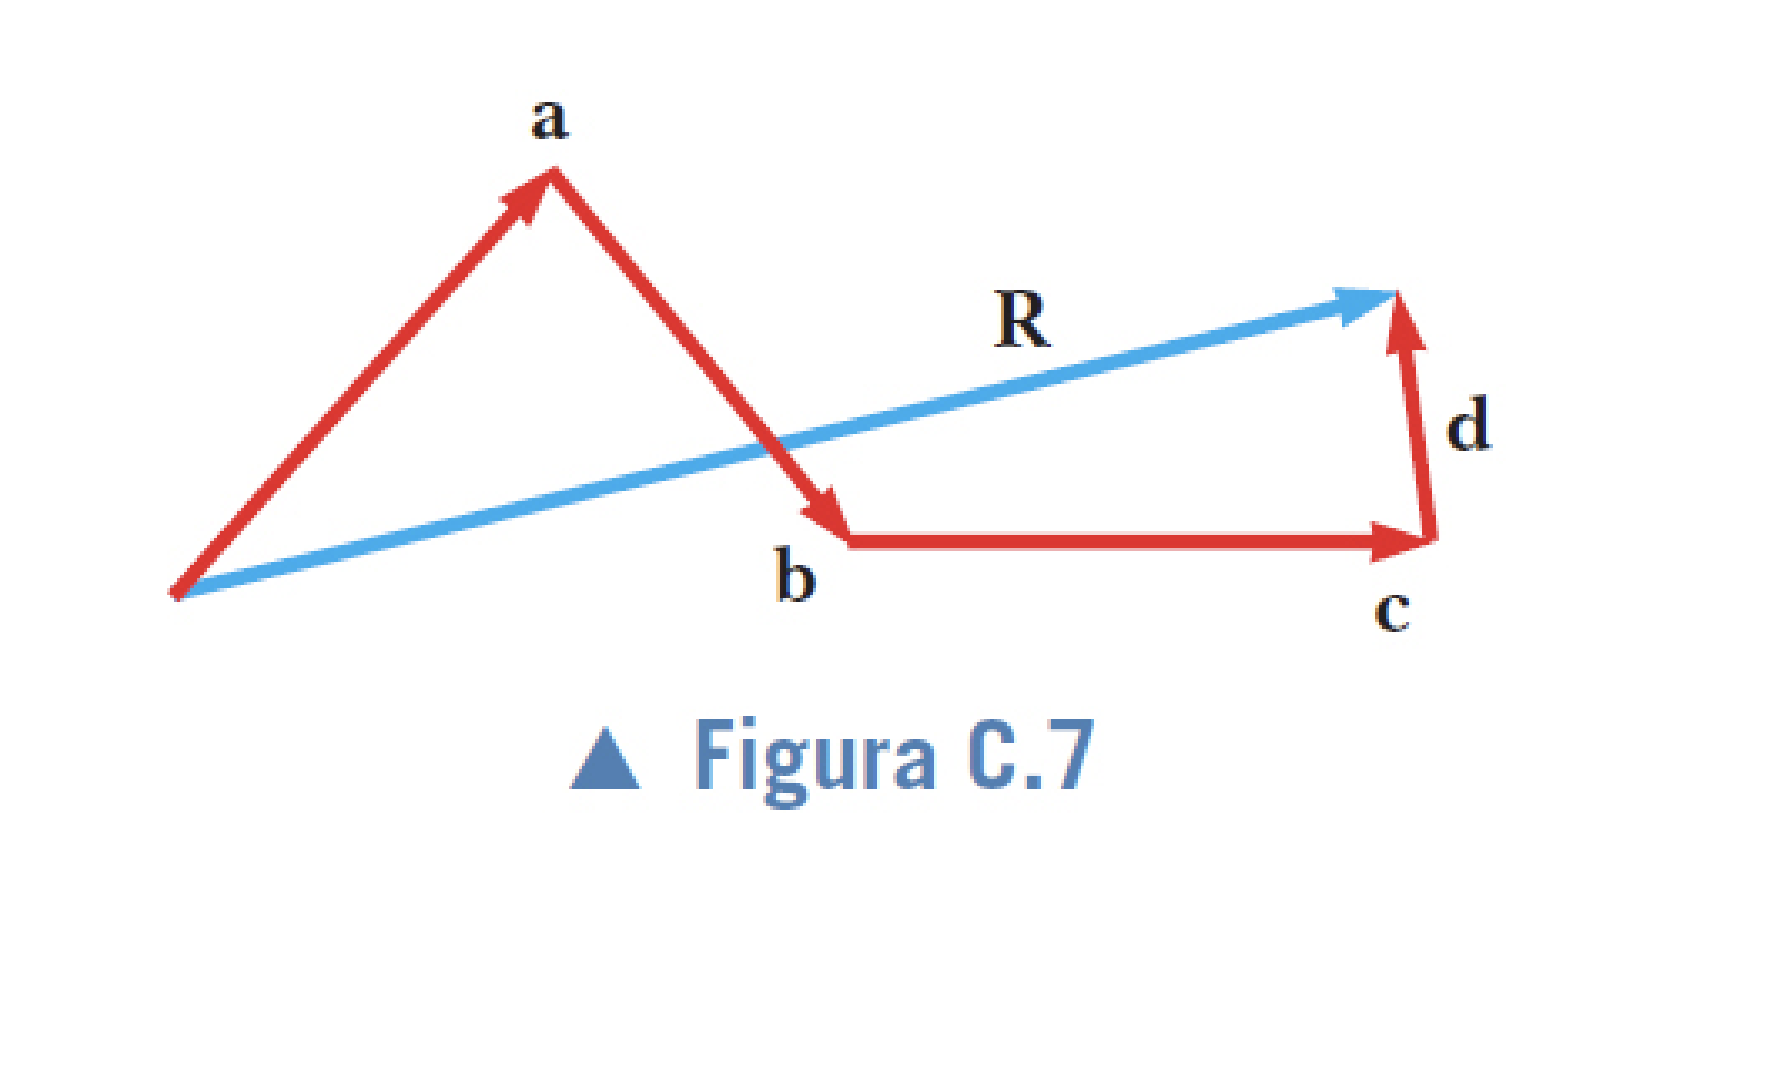
\includegraphics[width=0.5\textwidth]{Screenshot 2024-02-21 at 08.58.18.png}
        \caption{Somma di più vettori}
    \end{figure}
    \item \textbf{?}: $\vec{a_1} = a_1 \cdot \bar{u}_{a}$, $\vec{a} = a_2 \cdot \bar{u}_{a_2}$, $\vec{a_1} + \vec{a_2} = (a_1 + a_2) \cdot \bar{u}_{a}$
\end{itemize}
\subsubsection{Scomposizione di un vettore}
Ho un vettore che non è applicato in nessun punto, ponendolo all'interno del piano cartesiano posso scomporlo.
\[
    \vec{v} = \vec{v}_{xy} + \vec{v}_{z} = \vec{v}_{x} + \vec{v}_{y} + \vec{v}_{z} = v_x \cdot \bar{u}_x + v_y \cdot \bar{u}_y + v_z \cdot \bar{u}_z
\]
\begin{figure}[h!]
    \centering
    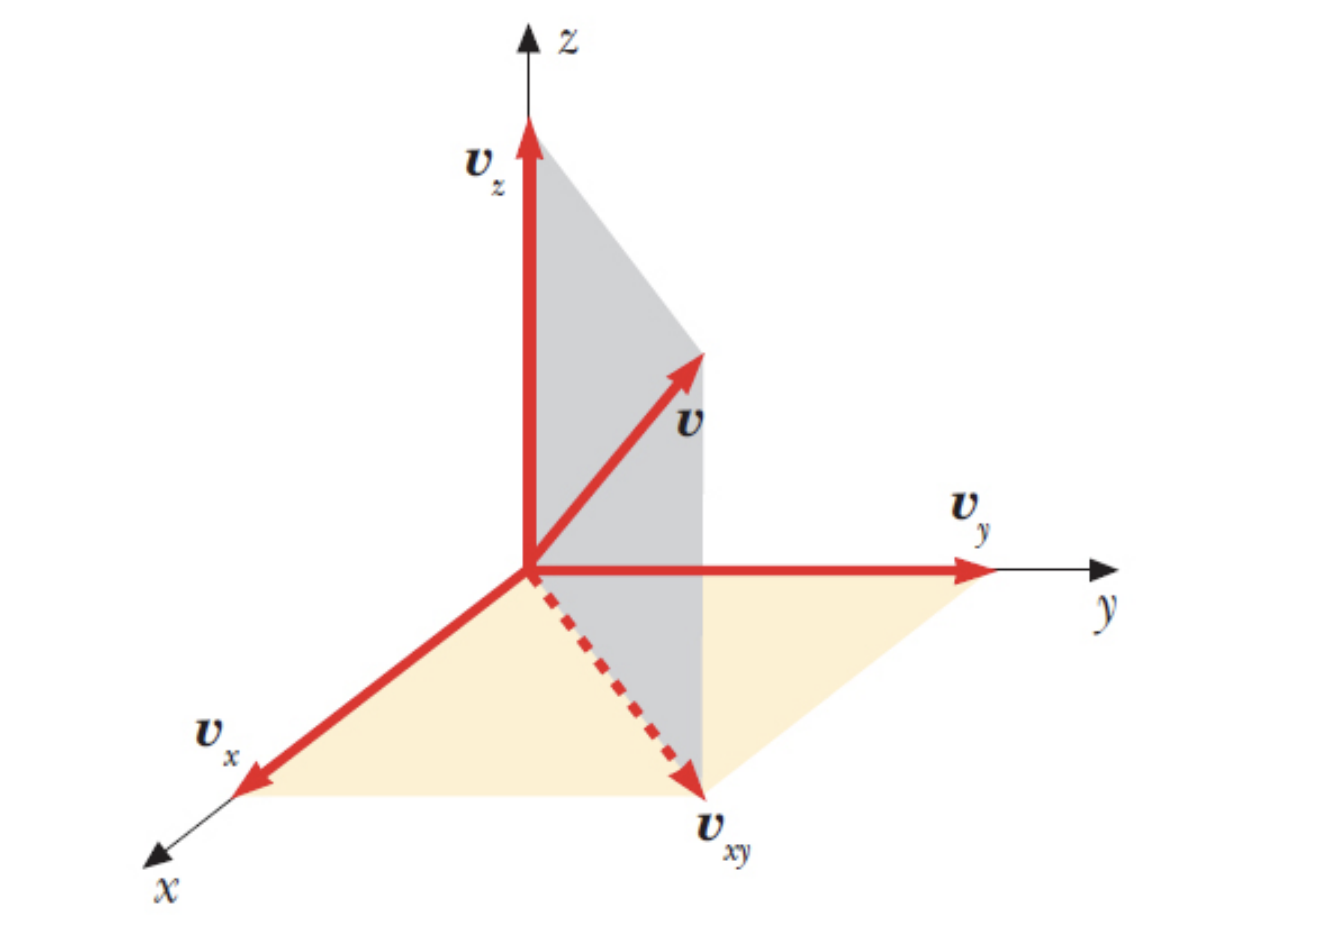
\includegraphics[width=0.5\textwidth]{scomposizione.png}
    \caption{Scomposizione di un vettore}
\end{figure}

Il vettore iniziale viene scomposto in componenti e ottengo una scrittura cartesiana del vettore.
\begin{itemize}
    \item \textbf{Vettore componente lungo l'asse $x$}: $\vec{v}_x$
    \item \textbf{Componente lungo l'asse $x$}: $v_x$
\end{itemize}
Una volta scomposto il vettore si può effettuare la somma dei vettori in maniera analitica. Per ciascuno ottengo le sue componenti cartesiane e successivamente sommo le componenti.
\[
    \vec{a} + \vec{b} = (a_x \cdot \bar{u}_x + a_y \cdot \bar{u}_y + a_z \cdot \bar{u}_z) + (b_x \cdot \bar{u}_x + b_y \cdot \bar{u}_y + b_z \cdot \bar{u}_z) = (a_x + b_x) \cdot \bar{u}_x + (a_y + b_y) \cdot \bar{u}_y + (a_z + b_z) \cdot \bar{u}_z
\]
\subsubsection{Prodotto scalare}
\[
    \vec{a} \bullet \vec{b} = \textit{ Scalare} \ \ \ \ |\vec{a}| = \textit{ Modulo} = ab \cos(\theta)
\]
Prodotto scalare tra due vettori:
\[
    |\vec{a}||\vec{b}| \cos(\theta)
\]
Il prodotto scalare è nullo quando i due vettori sono perpendicolari, il $\cos(\theta)$ è $0$.
\begin{enumerate}
    \item \textbf{Proprietà commutativa}: $\vec{a} \bullet \vec{b} = \vec{b} \bullet \vec{a}$
    \item $\vec{a} = \vec{b} \implies \vec{a} \bullet \vec{b} = |\vec{a}|^2$
    \item La proprietà associativa non vale perchè il prodotto scalare è definito solo tra vettori.
    \item \textbf{Proprietà distributiva}: $\vec{a} \bullet (\vec{b} + \vec{c}) = \vec{a} \bullet \vec{b} + \vec{a} \bullet \vec{c}$
    \item $(\vec{a} + \vec{b}) \bullet (\vec{a} + \vec{b}) = |\vec{a} + \vec{b}|^2 = \vec{a} \bullet \vec{a} + \vec{b} \bullet \vec{b} + \vec{a} \bullet \vec{b} + \vec{b} \bullet \vec{a} = \vec{a}^2 + \vec{b}^2 + 2\vec{a} \bullet \vec{b} \implies$ Teorema di Carnot.
    \item $\vec{a} \bullet \vec{b} = (a_x \cdot \bar{u}_x + a_y \cdot \bar{u}_y + a_z \cdot \bar{u}_z) \bullet (b_x \cdot \bar{u}_x + b_y \cdot \bar{u}_y + b_z \cdot \bar{u}_z) = FINIRE$
    \item $\vec{a} \bullet \vec{a} = a_x^2 + a_y^2 + a_z^2 \implies \ \ a = \sqrt{a_x^2 + a_y^2 + a_z^2}$
\end{enumerate}
\subsubsection{Prodotto vettoriale}
Il prodotto tra due vettori $\vec{a}$ e $\vec{b}$ è un vettore che giace al piano perpendicolare individuato da $\vec{a}$ e $\vec{b}$.
\[
    \vec{c} = \vec{a} \times \vec{b}
\]
\[
    |c| = |a||b| \sin(\theta)
\]
Regola della mano destra oppure vite destrorsa.
\begin{figure}[h!]
    \centering
    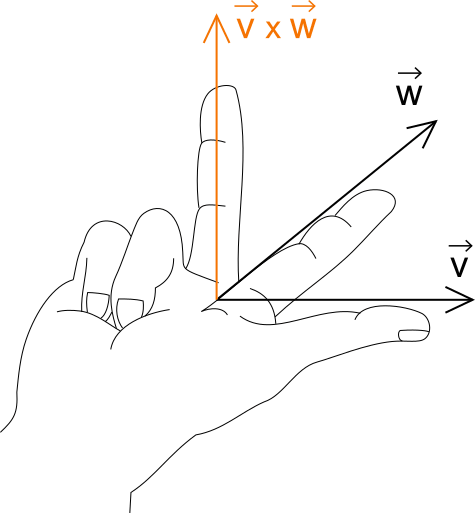
\includegraphics[width=0.3\textwidth]{manodx.png}
    \caption{Regola della mano destra}
\end{figure}

Il prodotto vettoriale non è commutitativo. E' \textbf{anticommutativo}; il vettore risultante ha la stessa direzione e lo stesso modulo ma verso opposto.
\[
    \vec{a} \times \vec{b} = - \vec{b} \times \vec{a}
\]
Vale la \textbf{proprietà distributiva}.
\[
    \vec{a} \times (\vec{b} + \vec{c}) = \vec{a} \times \vec{b} + \vec{a} \times \vec{c}
\]
Non vale la proprietà \textbf{associativa}.
\[
    (\vec{a}\times\vec{b})\times\vec{c} \neq \vec{a}\times(\vec{b}\times\vec{c})
\]
$\star$ Vedi il prodotto vettoriale di versori.
\subsection{Formuletta del profe}
Il prodotto vettoriale si può calcolare utilizzando le matrici.
\[
    A = \vec{c} = \begin{vmatrix}
        \bar{u}_x & \bar{u}_y & \bar{u}_z \\
        a_x & a_y & a_z \\
        b_x & b_y & b_z
    \end{vmatrix} = \vec{a} \times \vec{b}
\]
\[
    \det{A} = \vec{c} = \bar{u}_x(-1)^2(a_yb_z - a_zb_y) + \bar{u}_y(-1)^3(a_xb_z - a_zb_x) + \bar{u}_z(-1)^4(a_xb_y - a_yb_x)
\]

\subsection{Derivata di un vettore}
Per continuità possiamo definire la derivata di un vettore come la derivata a cui siamo abituati.
\[
    \lim_{h \to 0} \dfrac{f(x+h) - f(x)}{h} = f'(x) \ \textit{ per gli scalari}
\]
\[
    \lim_{\Delta t \to 0} \dfrac{\vec{x}(t + \Delta t) - \vec{x}(t)}{\Delta t} = \dfrac{d\vec{x}}{dt} \ \textit{ per i vettori}
\]
\begin{figure}[h!]
    \centering
    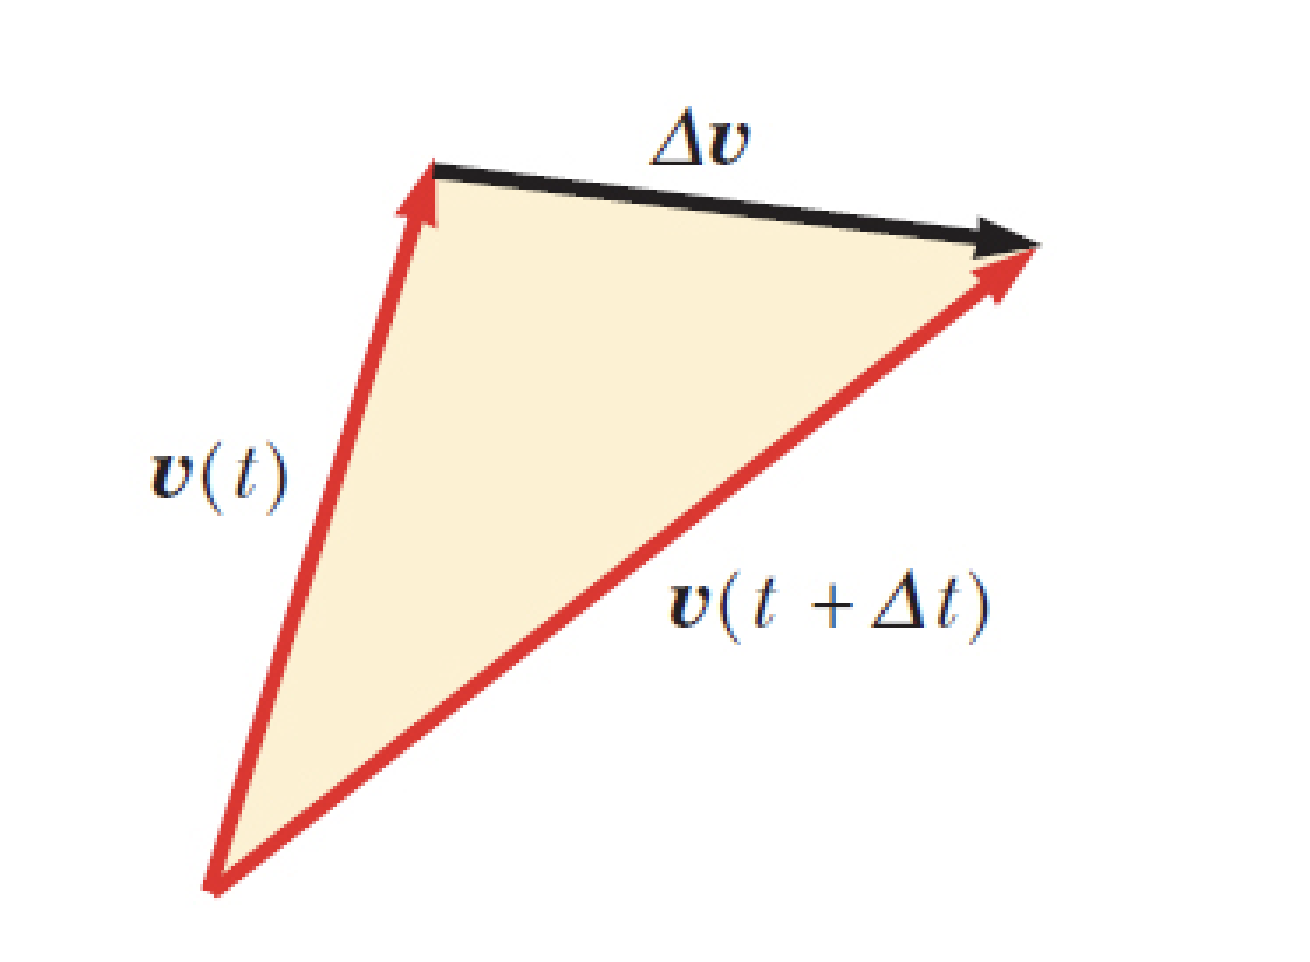
\includegraphics[width=0.3\textwidth]{derivata.png}
    \caption{Derivata di un vettore}
\end{figure}

\begin{itemize}
    \item $\dfrac{d(\vec{a} + \vec{b})}{dt} = \dfrac{d\vec{a}}{dt} + \dfrac{d\vec{b}}{dt}$
    \item $\dfrac{d}{dt} k\vec{a} = k\dfrac{d\vec{a}}{dt}$
    \item $\dfrac{d}{dt} (k\vec{a}) = \dfrac{dk}{dt}\vec{a} + k\dfrac{d\vec{a}}{dt}$
    \item $\dfrac{d}{dt} (\vec{a} \bullet \vec{b}) = \dfrac{d\vec{a}}{dt} \bullet \vec{b} + \vec{a} \bullet \dfrac{d\vec{b}}{dt}$
    \item $\dfrac{d}{dt} (\vec{a} \times \vec{b}) = \dfrac{d\vec{a}}{dt} \times \vec{b} + \vec{a} \times \dfrac{d\vec{b}}{dt}$
    \item se ho la scrittura cartesiana del vettore $\vec{a} = a_x\bar{u}_x + a_y\bar{u}_y + a_z\bar{u}_z$ allora $\dfrac{d\vec{a}}{dt} = \dfrac{da_x}{dt}\bar{u}_x + \dfrac{da_y}{dt}\bar{u}_y + \dfrac{da_z}{dt}\bar{u}_z$
\end{itemize}

\newpage
\subsection{Derivata di un versore}
La derivata del versore è differente in quanto nel tempo solo la direzione e il verso cambiano, non il modulo.
\begin{figure}[h!]
    \centering
    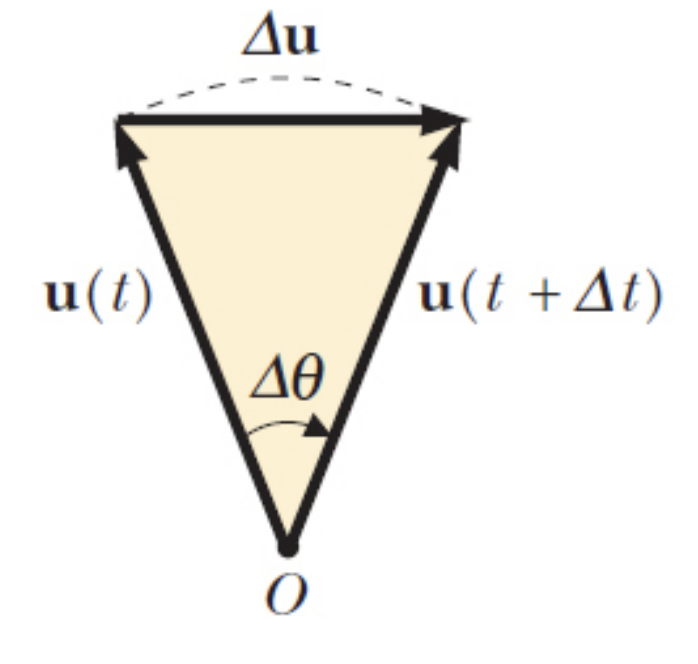
\includegraphics[width=0.3\textwidth]{versorederivata.png}
    \caption{Derivata di un versore}
\end{figure}
\[
    \Delta \bar{u} = \bar{u}(t+\Delta t) - \bar{u}(t)
\]
\[
    du = d\theta \cdot |u(t)|
\]
\[
    d\bar{u} = d\theta \cdot \bar{u}_n
\]
\[
    \dfrac{d\bar{u}}{dt} = \dfrac{d\theta}{dt} \cdot \bar{u}_n
\]

\begin{figure}[h!]
    \centering
    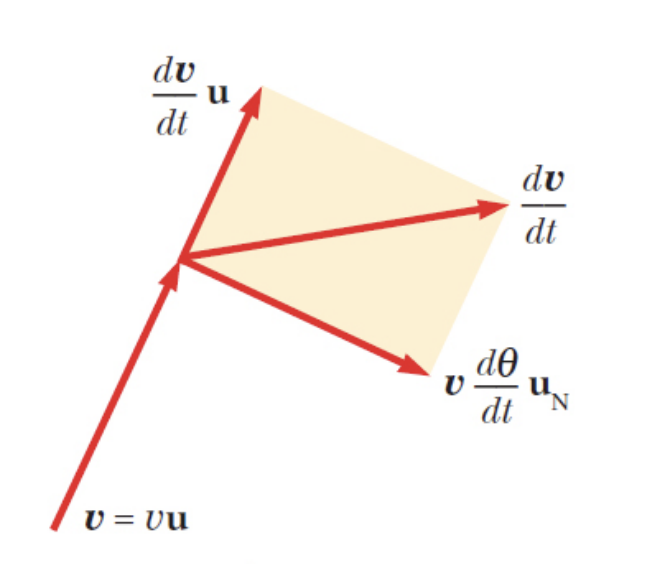
\includegraphics[width=0.3\textwidth]{verovettore.png}
\end{figure}

\[
    \vec{v} = v \cdot \bar{u} \implies \dfrac{dv}{dt} = \dfrac{d(v\bar{u})}{dt} + v\dfrac{d\bar{u}}{dt} = \dfrac{d(v\bar{u})}{dt} + v\dfrac{d\theta}{dt}\bar{u}_n
\]
\[
    |\dfrac{d\vec{v}}{dt}| = \sqrt{(\dfrac{dv}){dt})^2 + (\dfrac{vd\theta}{dt})^2}
\]

\subsection{}


\end{document}